\documentclass[a4paper]{article}
\linespread{1.6}
\usepackage{enumerate}
\usepackage{geometry}
\usepackage{setspace}
\usepackage{amsmath}
\usepackage{amssymb}
\usepackage[pdftex]{graphicx}
\usepackage{float}
\usepackage{subfigure}
\usepackage{listings}
\geometry{left=1.2cm,right=1.2cm,top=2.5cm,bottom=2.5cm}

\begin{document}
\begin{spacing}{2.0}
\begin{flushleft}\begin{huge}EEE6512 Image Processing and Computer Vision   Homework 2\end{huge}\end{flushleft}
\begin{flushright}\begin{Large} Hudanyun Sheng \end{Large}\end{flushright}

\section*{\huge\textbf{ Part \uppercase\expandafter{\romannumeral1} Textbook Questions}  }
	\normalsize
	
	\textbf{2-4} What are the actual names of the three types of cones, which are colloquially called red, green, and blue?
	
	The actual names of the three types of cones are L- cones, M - cones, and S - cones, correspond to long wavelength, middle 
	wavelength and short wavelength, respectively. Where L - cones is most sensitive to long-wavelength light, in which red light dominate; M - cones is 
	most sensitive to middle-wavelength light, in which green light dominate; and S - cones is most sensitive to short-wavelength light, in which blue light 
	dominate.\\
	
	\noindent
	\textbf{2-9} Match each term on the left with with the lighting condition on the right.
	\begin{center}
	scotopic vision    \qquad  \qquad   \qquad   \qquad   \qquad    sunlight\\
	photopic vision    \qquad  \qquad   \qquad   \qquad   \qquad    moonlight\\
	mesopic vision    \qquad  \qquad   \qquad   \qquad   \qquad    starlight\\
	\end{center}
	
	\noindent
	\textbf{2-10} Cones do not work in the dark, because they are not sensitive enough. What about the converse: Do rods produce meaningful signals 
	in everyday well-lit conditions? Why or why not?
	
	Rods do not produce meaningful signals in everyday well-lit conditions. Based on the text book, when it comes to everyday well-lit condition, the rods are saturated and the cones are mainly responsive.\\
	
	\noindent
	\textbf{2-22} Describe the essential elements of a pinhole camera.
	
	The essential elements of a pinhole camera are the focal point (the centre of projection) and the image plane.\\
	
	\noindent
	\textbf{2-24} Which has a longer wavelength: radio waves or X-rays? Which is more dangerous, and why?
	
	Compared between radio waves and X-rays, radio waves has a longer wavelength. X-rays is more dangerous, because shorter wavelength corresponds to larger energy, based on the formula $E = h\nu = hc/\lambda$, where h is the Planck's constant, c is the speed of light, which should be considered a constant when comparing two different waves, and $\lambda$ is the wavelength. So the longer the wavelength, the smaller the photon energy. \\
	
	\noindent
	\textbf{3-5} Use 8-bit saturation arithmetic to compute the following: (a) 52 + 200, (b) 86 + 199, (c) 30 - 50, and (d) 32 + 11. Then repeat with 4-bit saturation arithmetic.
	
	\textbf{Solution}:\\
	\textbf{8 - bit saturation arithmetic}: 
		\begin{enumerate}[(a)] 
			\item $52+200 = \mathbf{252}$.
			\item $86+199 = 285>255$, so we got  $\mathbf{255}$.
			\item $30-50 = -20$, so we got  $\mathbf{0}$.
			\item $32+11 =  \mathbf{43}$
		\end{enumerate}
	\textbf{4 - bit saturation arithmetic}: 
		$2^4-1 = 15$, so the largest value should be $15$.
		\begin{enumerate}[(a)] 
			\item $252>15$, so we got  $\mathbf{15}$.
			\item $285>15$, so we got  $\mathbf{15}$.
			\item $-20<0$, so we got  $\mathbf{0}$.
			\item $43>15$, so we got  $\mathbf{15}$.\\
		\end{enumerate}
	
	\noindent
	\textbf{3-7} Compute the (a) sum, (b) difference, and (c) absolute difference of the following two 8-bit images, using saturation arithmetic to store the result in another 8-bit image:\\
	\begin{center}
	$I_1 = \left[\begin{matrix} 19 & 171 & 91 & 68 \\ 123 & 99 & 74 & 195 \\ 85 & 71 & 208 & 18 \\ 241 & 212 & 189 & 68 \end{matrix}\right]$
	 \qquad  \qquad   \qquad
	$I_2 = \left[\begin{matrix} 106 & 97 & 190 & 5 \\ 81 & 64 & 183 & 82 \\ 71 & 200 & 251 & 94 \\ 181 & 76 & 9 & 18 \end{matrix}\right]$
	\end{center}
	
	\textbf{Solution}:
	\begin{enumerate}[(a)]
	\item $I_1 + I_2 =  \left[\begin{matrix} 125 & 255 & 255 & 73 \\ 204 & 163 & 255 & 255 \\ 156 & 255 & 255 & 112 \\ 255 & 255 & 198 & 86 \end{matrix}\right]$
	
	\item $I_1 - I_2 =  \left[\begin{matrix} 0 & 74 & 0 & 63 \\ 42 & 35 & 0 & 113 \\ 14 & 0 & 0 & 0 \\ 60 & 136 & 180 & 50 \end{matrix}\right]$
	
	\item $\left|I_1 - I_2\right| =  \left[\begin{matrix} 87 & 74 & 99& 63 \\ 42 & 35 & 109 & 113 \\ 14 & 129 & 43 & 76 \\ 60 & 136 & 180 & 50 \end{matrix}\right]$\\
	\end{enumerate}
	
	\noindent
	\textbf{3-8} Suppose you want to display the following floating-point image. Perform a linear contrast stretch to convert the pixels to 8 bits, mapping 
	the smallest value to 0 and the largest value to 255.
	$$\left[\begin{matrix} 0.327 & 0.945 & 0.559 & 0.381 \\ 0.181 & 0.252 & 0.080 & 0.950 \\ 0.240 & 0.399 & 0.737 & 0.148 \\ 0.986 & 0.170 & 0.246 & 0.447 \end{matrix}\right]$$
	
	\textbf{Solution}: $g_{min} = 0.080$, $g_{max} = 0.986$, based on equation (3.20) in the textbook:
	$$I'(x, y) = Round(255\times\displaystyle\frac{I(x,y) - g_{min}}{g_{max} - g_{min} })$$
	Where $I = \left[\begin{matrix} 0.327 & 0.945 & 0.559 & 0.381 \\ 0.181 & 0.252 & 0.080 & 0.950 \\ 0.240 & 0.399 & 0.737 & 0.148 \\ 0.986 & 0.170 & 0.246 & 0.447 \end{matrix}\right]$.\\
	With the help of MATLAB, I got $I = \left[\begin{matrix} 70 & 243 & 135 & 85 \\ 28 & 48 & 0 & 245 \\ 45 & 90 & 185 & 19 \\ 255 & 25 & 47 & 103 \end{matrix}\right]$.\\
	
	\noindent
	\textbf{3-12} Compute bit plane 7 and bit plane 4 for the image in Problem 3.1.\\
	The image in Problem 3.1: $$I = \left[\begin{matrix} 176 & 94 & 201 & 219 \\ 37 & 161 & 16 & 88 \\ 71 & 129 & 177 & 81 \\ 41 & 198 & 107 & 19\end{matrix}\right]$$
	\textbf{Solution}:\\
	\renewcommand\arraystretch{0.65}
	bit plane 7: 8 bits per pixel. $$\left[\begin{matrix} 1 & 0 & 1 & 1 \\ 0 & 1 & 0 & 0 \\ 0 & 1 & 1 & 0 \\ 0 & 1 & 0 & 0\end{matrix}\right]$$
	bit plane 4: 5 bits per pixel. $$\begin{bmatrix} 1 & 1 & 0 & 1 \\ 0 & 0 & 1 & 1 \\ 0 & 0 & 1 & 1 \\ 0 & 0 & 0 & 1\end{bmatrix}$$

	\noindent
	\textbf{3-13} Compute the histogram, normalized histogram, and cumulative normalized histogram for the following 4-bit image:	
	$$\begin{bmatrix} 5 \ \ & 8 \ \  & 3 \ \  & 7 \ \  \\ 1 \ \  & 3 \ \  & 3 \ \  & 9 \ \  \\ 6 \ \  & 8 \ \  & 2 \ \  & 7 \ \  \\ 4 \ \  & 1 \ \  & 0  \ \ & 9 \ \  \end{bmatrix}$$
	\textbf{Solution}: Since it is a 4-bit image, so there are $2^4 = 16$ possible gray levels.\\
	\textbf{Histogram}: $h = \begin{bmatrix} 1 & 2 & 1 & 3 & 1 & 1 & 1 & 2 & 2 & 2 \end{bmatrix}$, the subsequent 6 values are 0.\\
	\textbf{Normalized histogram}: $\bar{h} = h/16 = [0.0625 \quad 0.1250 \quad 0.0625 \quad 0.1875 \quad 0.0625 \quad 0.0625 \quad 0.0625 \quad 0.1250 \quad 0.1250 \quad 0.1250 \\ \quad 0 \quad 0 \quad 0 \quad 0 \quad 0 \quad 0 \quad]$\\
	\textbf{Cumulative normalized histogram}: $[[0.0625 \quad 0.1875 \quad 0.2500 \quad 0.4375 \quad 0.5000 \quad 0.5625 \quad 0.6250 \quad 0.7500 \quad 0.8750 \quad 1.0000 \\ \quad 1.0000  \quad 1.0000  \quad 1.0000  \quad 1.0000  \quad 1.0000  \quad 1.0000  \quad]$\\

\newpage	
\section*{\huge\textbf{ Part \uppercase\expandafter{\romannumeral2} MATLAB Programming} }
	
	\normalsize
	\begin{enumerate}
	\item The MATLAB code for the function``myhist" is attached. 
		\begin{figure}[H]
		    \centering
	    	    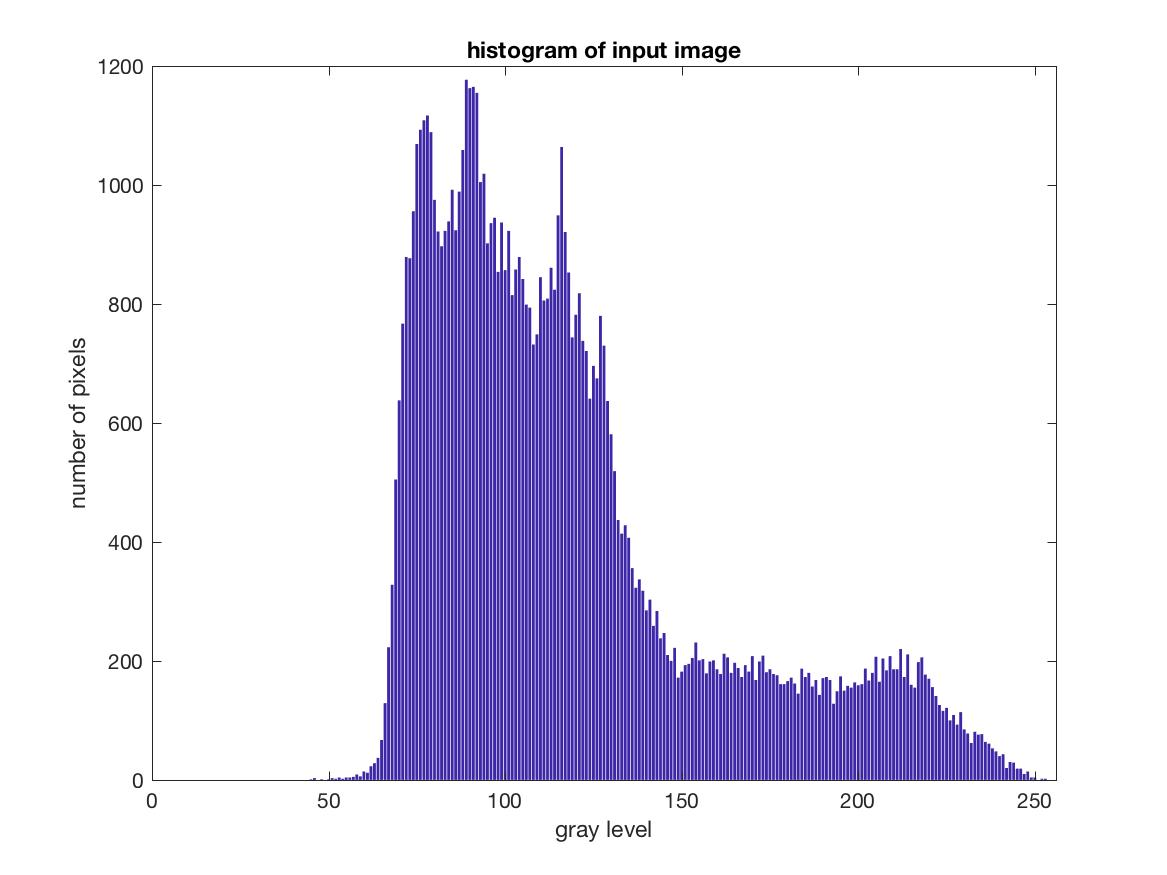
\includegraphics[width=4.5in]{1.jpg}
		    \caption{The histogram of the ``flower" image} 
	    	\end{figure}
	Based on the histogram of this ``\textbf{flower}" image, we can infer that this image has not high nor not low contrast. 
		
		\begin{figure}[H]
		    \centering
	    	    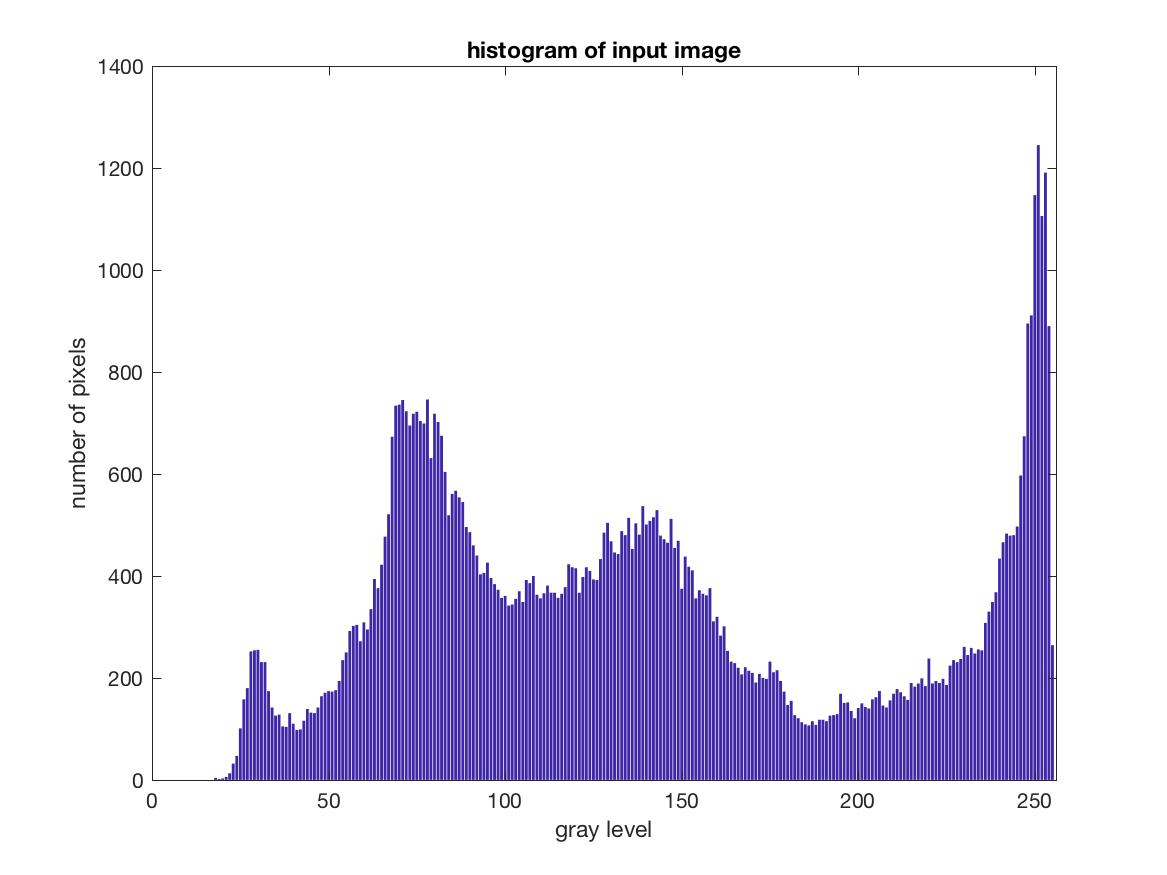
\includegraphics[width=4.5in]{2.jpg}
		    \caption{The histogram of the ``swan" image} 
	    	\end{figure}
	Based on the histogram of the ``\textbf{swan}" image, we can infer that this image has good exposure and has high contrast.
		
		\begin{figure}[H]
		    \centering
	    	    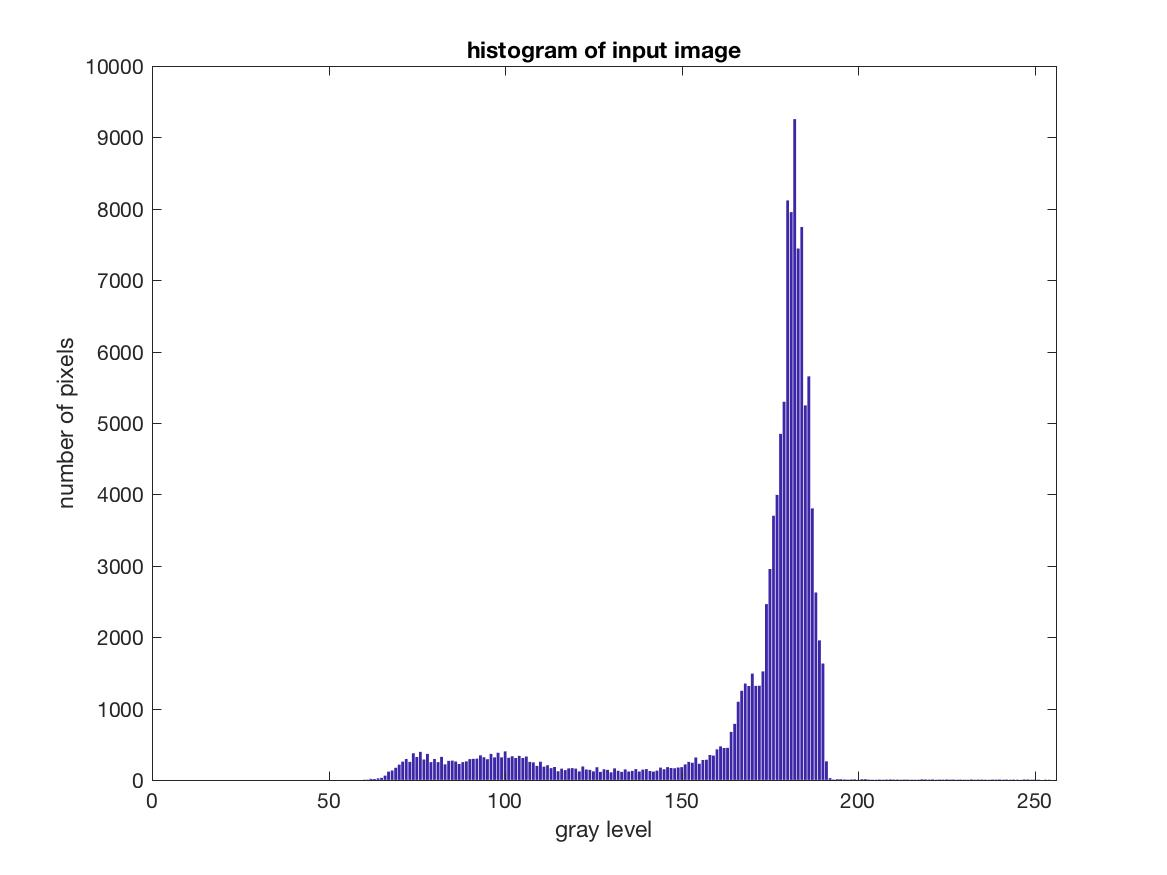
\includegraphics[width=4.5in]{3.jpg}
		    \caption{The histogram of the ``tools" image} 
	    	\end{figure}
	Based on the histogram of the ``\textbf{tools}" image, we can infer that this image has low contrast, and that it is not too dark nor too bright.\\
	
	
	\item The commented MATLAB code for the function ``myquantize" is attached.\\
		 Based on the basic idea of quantization, the number of gray levels equals the number of ``stairs" in the figure 3.16 in textbook.\\
		 The number of gray levels also equal to the intervals we need to have to segment the values of each pixel in the input image, from 0 to 255, 		 e.g. if the number of gray levels equals 8, that means we have to segment the values of each pixel in the input image into 8 intervals, from 0 		 to 255:\\
		 $[\mathbf{0}, 32)$, $[\mathbf{32}, 64)$, $[\mathbf{64}, 96)$, $[\mathbf{96}, 128)$, $[\mathbf{128}, 160)$, $[\mathbf{160}, 192)$, $				[\mathbf{192}, 224)$,  $[\mathbf{224}, 256)$ \\
		 And at the same time, the lower level of each interval is values that can appear in the output image. (As shown in bold in the above example).		\\
		 With these intervals on hand, the only thing we need to do is to traverse every gray level. For a specific gray level ``iter", we want to find the 			pixels in the original image which are in the iter-th interval: lower level of interval $\leq$value of the pixel $\mathbf{<}$ higher level, and replace the values of these pixels with the lower level of the iter-th interval.\\
		 To sum up, the basic calculations in my own function of quantization looks like this:\\
		 $quant\_num =$ number of gray levels\\
		 $step =256/quant\_num$. Based on the step, we can calculate a vector that every number in that vector is the start and/or end point for the 		bins. The vector for the former example would be $\left[\begin{matrix} \mathbf{0} & \mathbf{32} & \mathbf{64} & \mathbf{96} & \mathbf{128} & 			\mathbf{160} & \mathbf{192} & \mathbf{224} & 256 \end{matrix}\right]$. This vector with 9 values has 8 intervals, and the former 8 values(bolded) are 	the values which appears in the output image. \\
		Then we can traverse every gray level as described above to got the output image.
	
	\end{enumerate}



	
\end{spacing}
\end{document}